\documentclass[standalone]{subfiles}

\begin{document}

\chapter{Marco de Trabajo (Framework)}
\label{ch:framework}

\section{Introducción}
La instrumentación científica en laboratorios de física experimental enfrenta frecuentemente el desafío de la falta de reproducibilidad y el empaquetamiento propietario...

\section{Marco Teórico}
\subsection{Paradigma de Co-diseño Hardware/Software}
\subsection{Filosofía y Ecosistema PYNQ}
\subsection{Filosofía y Gestión DevOps con Hog}

\section{Metodología}
\subsection{Estrategia de Repositorios Duales (HW/SW)}
\subsection{Flujo de Trabajo CI/CD y Transducción AXI/DMA}
\subsection{Justificación: Instrumentación Libre, Modular y Reusable}

\section{Resultados y Validación}
\subsection{Plataforma de Adquisición: \texttt{hw-xadc-dma-overlays}}
\label{subsec:hw_overlay}

Para validar el marco de trabajo propuesto y establecer un entorno preliminar de pruebas para sistemas de adquisición de datos (DAQ), se desarrolló el repositorio de firmware \texttt{hw-xadc-dma-overlays}, orientado a la tarjeta SoC-FPGA PYNQ-Z2 (dispositivo Zynq-7000 \texttt{xc7z020clg400-1}). Este proyecto implementa una plataforma de adquisición en la Lógica Programable (PL) capaz de digitalizar señales analógicas en tiempo real y transferirlas hacia la memoria DDR del procesador (PS) sin intervención de la CPU.

\begin{figure}[htbp]
    \centering
    \IfFileExists{figures/xadc_bd_diagram.png}{%
        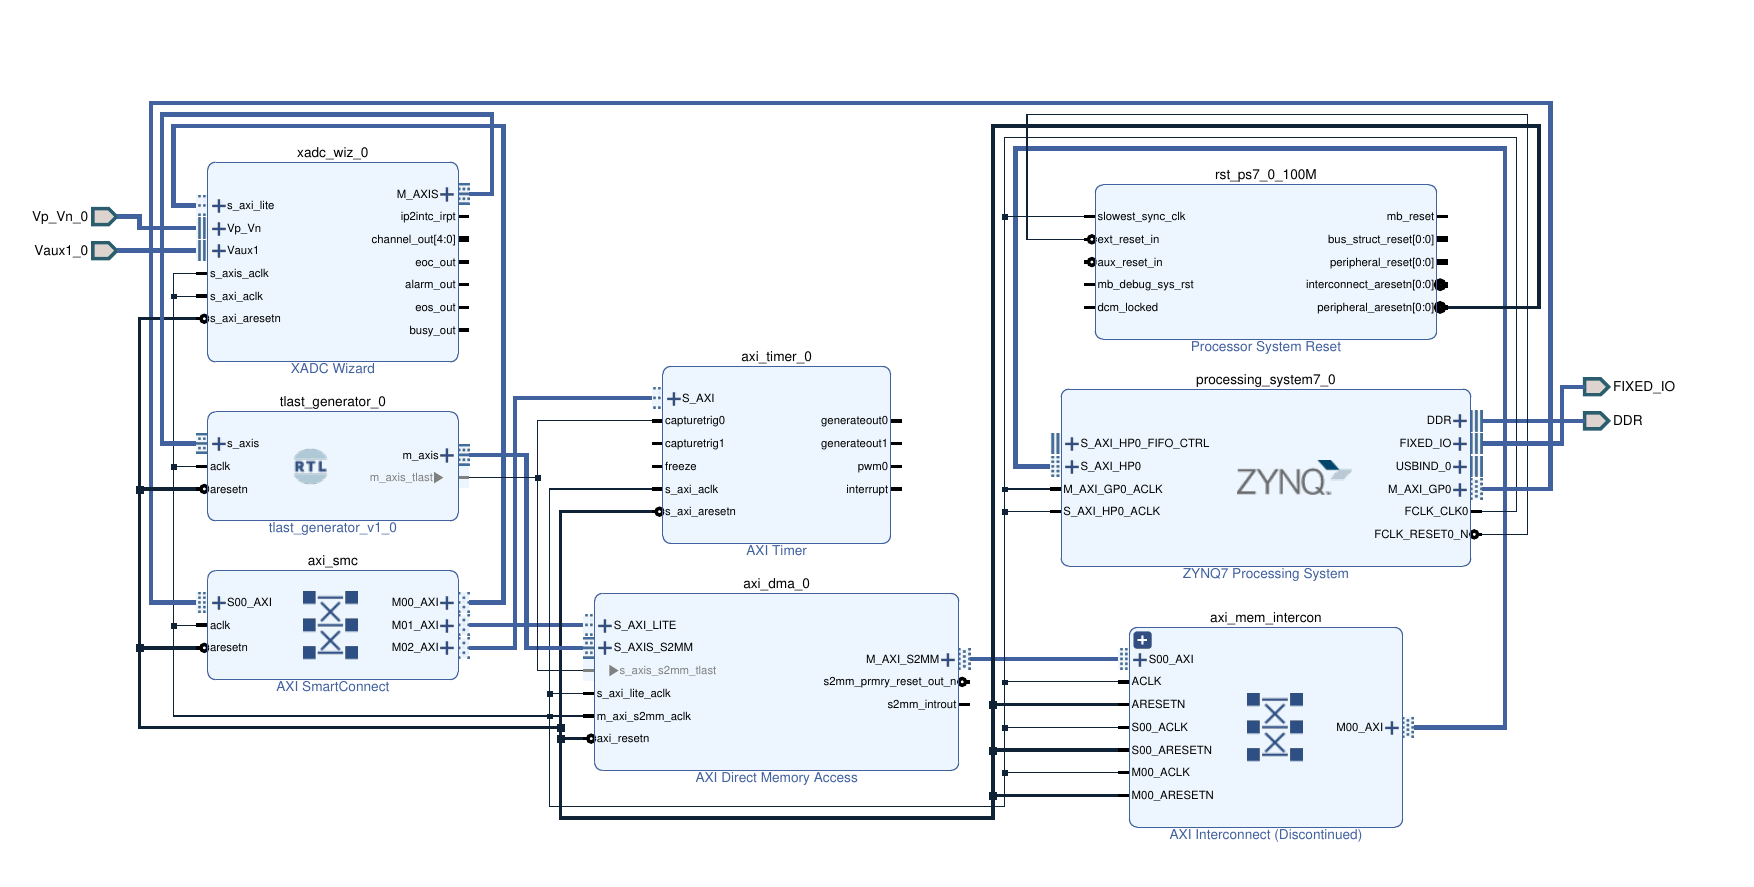
\includegraphics[width=\textwidth]{figures/xadc_bd_diagram.png}%
    }{%
        \framebox[\textwidth][c]{%
            \parbox[c][6cm]{0.9\textwidth}{%
                \centering \textbf{[ Diagrama de Bloques en Vivado ]}\\[0.5em]
                \small (Agregue la imagen \texttt{xadc\_bd\_diagram.png} en la carpeta \texttt{figures/})%
            }%
        }%
    }
    \caption{Diagrama de bloques general en Vivado IP Integrator para la plataforma de adquisición \texttt{hw-xadc-dma-overlays}.}
    \label{fig:xadc_bd_diagram}
\end{figure}

\subsubsection{Arquitectura de Adquisición y Flujo AXI4-Stream}
La arquitectura de adquisición se diseñó utilizando Vivado 2024.2.2 bajo la metodología de IP Integrator (Figura~\ref{fig:xadc_bd_diagram}). El flujo de señal se articula a través de los siguientes módulos principales:

\begin{enumerate}
    \item \textbf{Digitalizador XADC (\texttt{xadc\_wiz\_0}):} Configurado en modo de canal único sobre la entrada auxiliar diferencial \texttt{VAUXP1/VAUXN1} (con opción a canal dedicado \texttt{VP/VN}), operando a una frecuencia de muestreo de $1~\text{MSPS}$ (1000~kSPS). La interfaz de salida fue establecida en formato AXI4-Stream de 16 bits (\texttt{M\_AXIS}).
    \item \textbf{Generador de TLAST (\texttt{tlast\_generator}):} Debido a que el bloque nativo XADC no genera la señal de final de paquete (\texttt{TLAST}), se diseñó un módulo VHDL personalizado que actúa como un empaquetador de flujo. Este módulo incrementa un contador síncrono en cada ciclo válido y aserta la señal \texttt{TLAST} combinacionalmente cada $N = 16\,384$ muestras (\texttt{PACKET\_SIZE}), delimitando los bloques de memoria requeridos por el motor DMA.
    \item \textbf{Acceso Directo a Memoria (\texttt{axi\_dma\_0}):} El motor AXI DMA opera en modo \textit{Simple DMA} directo (S2MM: \textit{Stream-to-Memory-Mapped}) con un tamaño de ráfaga (\textit{burst size}) de 128 transferencias. Los datos son transmitidos a través del interconector de datos (\texttt{axi\_mem\_intercon}), el cual adapta el flujo de 32 bits del DMA hacia el bus de alto rendimiento AXI-HP0 de 64 bits del Zynq PS. Aunque la CPU ARM Cortex-A9 opera a 32 bits, la transferencia de datos se realiza mediante DMA directamente hacia la memoria RAM compartida (\texttt{0x00000000} -- \texttt{0x1FFFFFFF}) sobre el bus de 64 bits, liberando por completo a la CPU de tareas de procesamiento de muestras en tiempo real.
    \item \textbf{Temporizador AXI y Medición de Latencia (\texttt{axi\_timer\_0}):} Como bloque de apoyo para caracterización, se integró un temporizador AXI cuya entrada de captura (\texttt{capturetrig0}) se encuentra interconectada directamente a la señal \texttt{TLAST}. Esto permite medir con precisión de ciclos de reloj ($10~\text{ns}$ a $100~\text{MHz}$) la latencia entre paquetes de adquisición desde el hardware.
    \item \textbf{Infraestructura de Interconexión y Reloj:} El bloque \texttt{processing\_system7\_0} genera un reloj de sistema de $100~\text{MHz}$ (\texttt{FCLK\_CLK0}) y un reseteo sincronizado mediante el bloque \texttt{rst\_ps7\_0\_100M}. La distribución de comandos de control desde el PS se gestiona mediante el conmutador AXI SmartConnect (\texttt{axi\_smc}) sobre el bus \texttt{M\_AXI\_GP0}, mapeando las direcciones de registro del DMA (\texttt{0x40400000}), del temporizador (\texttt{0x42800000}) y del XADC (\texttt{0x43C00000}).
\end{enumerate}

\subsubsection{Gestión de Firmware y Automatización con CERN Hog}
La construcción y control de versiones del proyecto de hardware se gestionaron mediante la herramienta CERN Hog. La estructura del repositorio se organiza bajo el directorio \texttt{Top/pynq\_z2/}, utilizando archivos de listas (\texttt{.src}) para desacoplar el código fuente VHDL y el diagrama de bloques (\texttt{xadc.bd}) de los archivos binarios propietarios de Vivado.

Adicionalmente, el \textit{wrapper} de nivel superior (\texttt{xadc\_wrapper.vhd}) incorpora genéricos de versión (\texttt{GLOBAL\_VER}, \texttt{GLOBAL\_SHA}), lo que permite embeber dinámicamente el \textit{hash} del commit de Git dentro de los registros del hardware durante la síntesis.

Al finalizar la implementación, un script de gancho (\textit{hook}) en TCL (\texttt{post-bitstream.tcl}) extrae el archivo de mapa de bits (\texttt{pynq\_z2.bit}) y el archivo de descripción de hardware (\texttt{pynq\_z2.hwh}) hacia la carpeta \texttt{bin/}. Finalmente, un flujo de integración continua en GitHub Actions (\texttt{release.yml}) empaqueta y publica automáticamente estos artefactos binarios en los lanzamientos del repositorio al detectar una etiqueta de versión (\texttt{v*}).

\subsection{Interfaz e Instrumentación: \texttt{sw-pynq-oscilloscope}}
\subsection{Proyección a Módulos de Localización Espacial}

\section{Conclusiones del Capítulo}

\end{document}